%Background image credits:https://commons.wikimedia.org/wiki/File:Hemp_paper_in_Japan.jpg タバコはマーダー, CC BY-SA 4.0, via Wikimedia Commons
%Background image credits:https://commons.wikimedia.org/wiki/File:Cannabis_Grandes_Heures_Anne_de_Bretagne_femelle_m%C3%A2le_1.jpg Jean Bourdichon , Public domain, via Wikimedia Commons
%Background image credits:https://commons.wikimedia.org/wiki/File:Seshat_emblem.svg Thetrueangel, CC BY-SA 4.0, via Wikimedia Commons
\documentclass[a4paper, 11pt, oneside, polutonikogreek]{article}
\usepackage[T1]{fontenc}
\usepackage{drm}
% Load encoding definitions (after font package)
\usepackage[dvipsnames]{xcolor}
\usepackage{eso-pic,graphicx}
%\usepackage[top=55mm, bottom=25mm, outer=18mm, inner=18mm]{geometry}
\setlength{\columnsep}{90pt}
\definecolor{customColor}{RGB}{0, 100, 0}

\usepackage{textalpha}

\usepackage{listings}
\lstset{basicstyle=\ttfamily}

% Babel package:
\usepackage[french]{babel}

% With XeTeX$\$LuaTeX, load fontspec after babel to use Unicode
% fonts for Latin script and LGR for Greek:
\ifdefined\luatexversion \usepackage{fontspec}\fi
\ifdefined\XeTeXrevision \usepackage{fontspec}\fi

% "Lipsiakos" italic font `cbleipzig`:
\newcommand*{\lishape}{\fontencoding{LGR}\fontfamily{cmr}%
		 \fontshape{li}\selectfont}
\DeclareTextFontCommand{\textli}{\lishape}

\usepackage{booktabs}
\setlength{\emergencystretch}{15pt}
\usepackage{fancyhdr}
\usepackage{microtype}

\usepackage{setspace}
\onehalfspacing

% change color of text, example replace all \color{Goldenrod} with \color{lightgray}

\makeatletter % change only the display of \thepage, but not \thepage itself:
\patchcmd{\ps@plain}{\thepage}{\color{customColor}{\thepage}}{}{}
\makeatother

\color{customColor}

\begin{document}
\AddToShipoutPictureBG{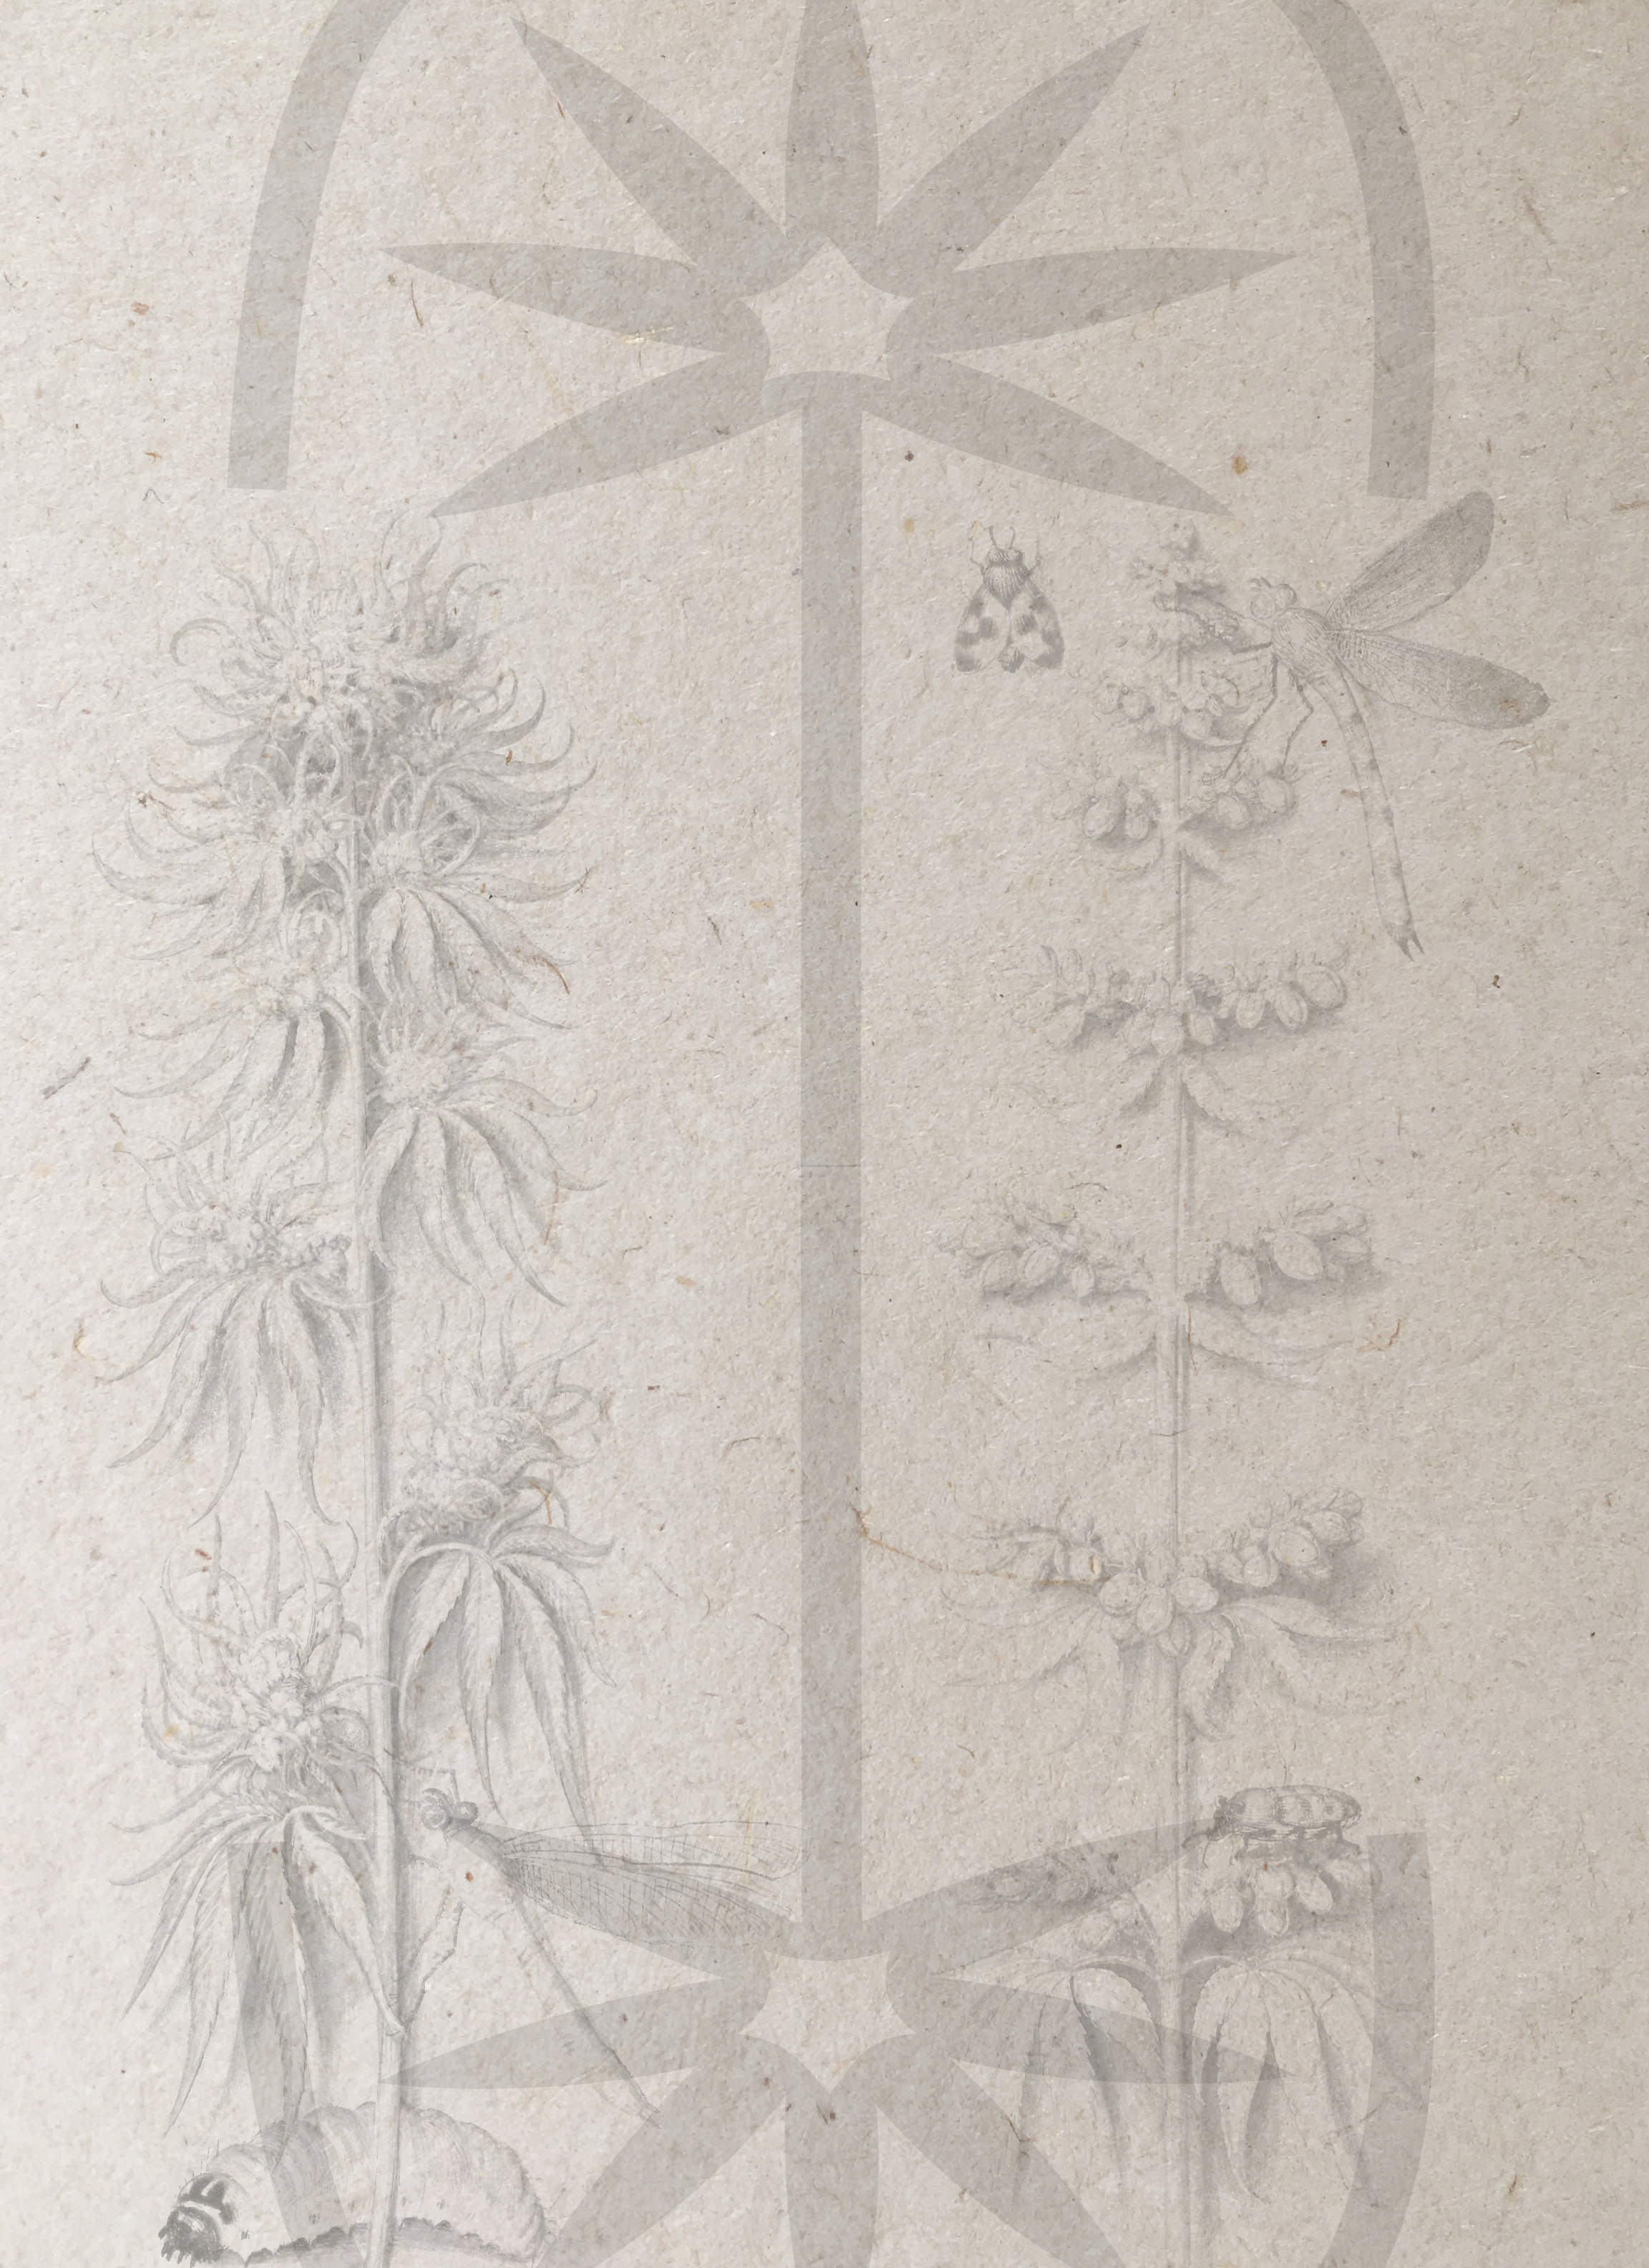
\includegraphics[width=\paperwidth,height=\paperheight]{Hemp_paper_in_Japan-canna5.jpeg}}
\begin{titlepage} % Suppresses headers and footers on the title page
	\centering % Centre everything on the title page
	%\scshape % Use small caps for all text on the title page

	%------------------------------------------------
	%	Title
	%------------------------------------------------
	
	\rule{\textwidth}{1.6pt}\vspace*{-\baselineskip}\vspace*{2pt} % Thick horizontal rule
	\rule{\textwidth}{0.4pt} % Thin horizontal rule
	
	\vspace{1\baselineskip} % Whitespace above the title
	
	{\scshape\Huge Recherches sur l'Emploi du Chanvre dans l'Antiquité et dans le Moyen Âge,}
	
	\vspace{1\baselineskip} % Whitespace above the title

	\rule{\textwidth}{0.4pt}\vspace*{-\baselineskip}\vspace{3.2pt} % Thin horizontal rule
	\rule{\textwidth}{1.6pt} % Thick horizontal rule
	
	\vspace{1\baselineskip} % Whitespace after the title block
	
	%------------------------------------------------
	%	Subtitle
	%------------------------------------------------

 	\vspace*{1\baselineskip} % Whitespace under the subtitle

	{\scshape \Large Par le citoyen Antoine Mongez.} % Subtitle or further description

 	\vspace*{1\baselineskip} % Whitespace under the subtitle

	%------------------------------------------------
	%	Editor(s)
	%------------------------------------------------
\vspace*{\fill}

	\vspace{1\baselineskip}

	{\small\scshape A Paris, Août 1800.}
		
	\vspace{0.5\baselineskip} % Whitespace after the title block

\scshape Internet Archive Online Edition% Publication year
	
	{\scshape\small Utilisation non commerciale --- Partage dans les mêmes conditions 4.0 International} % Publisher
\end{titlepage}
\setlength{\parskip}{1mm plus1mm minus1mm}
\clearpage
\begin{center}
Lu en fructidor an 9.
\end{center}
\paragraph{}
Il paraît que le chanvre n'était pas connu des Grecs, ou du moins qu'ils l'employaient peu au temps où Homère écrivait. On ne trouve le nom de ce végétal dans aucun des poèmes d'Hésiode ni dans ceux du chantre d'Achille. Celui-ci au contraire parle souvent du lin et de cuirasses de lin. C'était dans une toile de lin qu'Ulysse dormait enveloppé lorsque les Phéaciens le déposèrent sur les bords d'Ithaque, auprès de l'antre des nymphes. (Odyss. lib. 13, v. 117.)
\begin{quotation}
%ω used due to font issues with ῷ
Πρῶτον Ὀδυσσῆα γλαφυρῆς ἐκ νηὸς ἄειραν,

Αὐτῶ σύν τε λίνω, κὴ ρήγεΐ σιγαλεόντι,

Κἀδ᾽ δ᾽ ἄῤ ἐπὶ ψαμάθω ἔθεσαν, δεδμημένον ὕπνω.
\end{quotation}
\paragraph{}
Hérodote, qui écrivait dans le quatrième siècle avant l'ère vulgaire, est, à ma connaissance, le plus ancien auteur qui ait parlé du chanvre. (Lib. 4, sect. 74, p. 314, edit. Wesseling.) « Il croît en Scythie du chanvre (traduction de notre confrère Larcher, Paris, 1786) ; il ressemble fort au lin, excepté qu'il est plus gros et plus grand. Il lui est en cela de beaucoup supérieur. Cette plante vient d'elle-même et de graine. Les Thraces s'en font des vêtements qui ressemblent tellement à ceux du lin qu'il faut s'y bien connaître pour les distinguer, et quelqu'un qui n'en aurait jamais vu de chanvre, les prendrait pour des étoffes de lin ... » Ἔστι δὲ σφι κάνναβις φυομένη ἐν τῇ χώρη, πλὴν παχύτητος κὴ μεγάθεος, τῶ λίνω ἐμφερεστάτη · ταύτῃ δὲ πολλῶ ὑπερφέρει ἡ κάνναβις αὕτη · κὴ αὐτομάτη κὴ σπειρομένη φύεται · κὴ ἐξ αὐτῆς Θρήϊκες μὲν κὴ εἵματα ποιεῦνται τοῖσι λινέοισι ὁμοιότατα · οὐδ᾽ ἄν, ὃστις μὴ κάρτα τρίβων ἔιη αὐτῆς, διαγνοίη λίνου ἥ καννάβιὸς ἐστι · ὃς δὲ μὴ εἶδέκω τὴν καννάβιδα, λίνεον δοκήσει εἶναι τὸ εἶμα.

Il fallait qu'Hérodote n'eût jamais vu de chanvre pour annoncer aussi positivement dans son port quelque ressemblance avec celui du lin, indépendamment de la grosseur et de la hauteur. En effet, la différence de ces deux végétaux ne résulte pas uniquement de caractères difficiles à saisir, tels que peuvent en présenter les étamines, la forme du calice, \emph{etc.} ; mais il est facile de l'établir sur le port entier de l'une et de l'autre plante. La tige du lin est lisse, celle du chanvre est velue ; les feuilles du lin sont simples, celles du chanvre sont digitées, c'est-à-dire composées de folioles assemblées, souvent au nombre de cinq, comme les doigts de la main. Le lin est un sous-arbrisseau dans quelques espèces, et le chanvre est toujours herbe. La fleur du lin, fleur qui renferme les deux sexes, ressemble à celle des caryophyllées en général ou à celle de l'œillet en particulier, et sa couleur est variable. Le chanvre est dioïque, c'est-à-dire qu'il a ses deux sexes placés sur des individus séparés, et ses fleurs mâles sont constamment jaune-verdâtres, tandis que les femelles sont toujours d'un blanc sale. Voilà des caractères différentiels très-apparents qui auraient frappé Hérodote s'il eût vu les deux végétaux.

Théophraste, qui vivait un siècle après Hérodote, ne le connaissait probablement pas ; car il n'en fait aucune mention dans les livres qu'il a écrits sur les végétaux, et dans lesquels il parle du lin et du lin-sparte. Trois siècles après Théophraste, Dioscoride fut le premier des écrivains grecs parvenus jusqu'à nous qui, depuis Hérodote, parlât du chanvre. Il le décrit dans son livre 3 (chap. 165), mais sans désigner les contrées où on le cultivait, et il rapporte ses usages médicinaux, après avoir dit qu'il est employé à faire les cordes les plus fortes ... Πρὸς τὰς τῶν ἐυτονώτατων σχοινίων πλοκὰς ... Dans le chapitre suivant il nous instruit davantage : il nous apprend que c'était avec son écorce que l'on fabriquait ces cordes ... Καὶ ὁ ἀπὸ ταυτὴς δὲ φλοιὸς, εὔθετος εἰς πλοκὴν σχοινίων.

Pausanias décrivant l'Élide cent ans après l'époque où Dioscoride écrivait, dit que « le chanvre, le lin et le coton étaient cultivés par ceux de ses habitants qui occupaient un terrain favorable à ces cultures ... » Τὴν μὲν δὴ κανναβίδα καὶ λίνον, καὶ τὴν βύσσον σπείρουσιν ὅσοις ἡ γῆ τρέφειν ἐστιν ἐπιτήδειος ... C'est la première fois qu'il est fait mention de chanvre cultivé dans la Grèce.

Lorsque les Grecs eurent connu le chanvre, il ne paraît pas qu'ils l'aient employé à faire de la toile, comme le pratiquaient les Thraces dès le temps d'Hérodote ; du moins aucun écrivain de cette nation ne parle de tissus de chanvre. Ils en fabriquaient seulement des cordes, ou ils l'employaient en étoupe, si l'on en croit Varron, cité par Aulu-Gelle (lib. 17, cap. 3). « Les Liburniens, dit-il, assemblaient le plus souvent les bordages de leurs navires avec dès l’arrières de cuir. Les Grecs employaient de préférence à cet usage le chanvre et l'étoupe, et d'autres végétaux qu'ils désignaient par le mot σπαρτα ... » \emph{Liburni plerasque naves loris suebant. Græci magis cannabo et stupâ, cæterisque sativis rebus, à quibus σπαρτα appellabant.}

Athénée décrit (liv. 5, cap. 10) le navire qu'Hiéron avait fait construire pour un roi d'Égypte dans le troisième siècle avant l'ère vulgaire, navire célèbre dans l'antiquité par sa grandeur et sa magnificence ; il dit que le roi de Syracuse avait tiré les bois de la Sicile et de l'Italie ; d'Ibérie les cordages, qui étaient probablement de sparte ; « le chanvre et le lierre, des bords du Rhône ... » Κάνναβιν δὲ καὶ κίττον ἐκ τοῦ Ῥοδανοῦ, ποταμοῦ ... Eustathe, le scoliaste d'Homère, cite le passage d'Athénée en d'autres termes. (Casaub. \emph{Animadv. in lib. 5, cap. 10 Athenæi}) : Κάνναβιν δ᾽ ἐκ τοῦ Ἠριδανοῦ ποταμοῦ « le chanvre des bords de l'\emph{Eridanus}. » Il n'est fait ici mention que du chanvre ; mais c'est des bords de l'\emph{Eridanus} qu'il est tiré, et non des Gaules. Ces différences n'affectent point le résultat que je veux obtenir du texte d'Athénée ; j'y vois seulement une nouvelle preuve que les Grecs employaient le chanvre pour étouper les joints des navires, car on y trouve la matière des cordages énoncée dans la phrase précédente : ce qui semble restreindre l'usage du chanvre au calfatage.

Le nom du fleuve qui avait vu croître le chanvre employé par Hiéron, l'\emph{Eridanus}, a donné lieu à tant de fables et de contradictions, que l'on ne pourra me savoir mauvais gré d'avoir rapporté ce qu'écrivait à ce sujet en 1768 M. de la Nauze, dans les \emph{Recueils de l'Académie des belles lettres} (t. 36, p. 66). « Hérodote dit (c'est le savant académicien qui parle) que, malgré toutes ses recherches en Asie et dans la Grèce, il ne put trouver personne qui eût vu les îles Cassitérides d'où venait l'étain, ni l'\emph{Eridanus} d'où venait l'ambre. On sait depuis longtemps que les îles Cassitérides sont les îles Britanniques, et l'on présume que l'\emph{Eridanus} est ici la Rhodaune, rivière de Prusse. Apparemment que les marchands phéniciens faisaient mystère de la position des îles et du fleuve ; en conséquence Hérodote refuse d'en reconnaître l'existence : c'était aller trop loin. Pline, prenant cet \emph{Eridanus} pour le Pô, tomba dans une autre méprise. Il est fort étonnant, dit-il, ce que nous croyons pourtant sur la parole d'Hérodote, que l'Asie, la Grèce, Hérodote lui-même, ne connussent personne qui eût vu le Pô, \emph{etc.} \emph{etc.} »

Notre confrère Larcher a adopté la même opinion : il pense qu'Hérodote, en nommant l'\emph{Eridanus}, sur les bords duquel on trouvait l'ambre, voulait parler de le Rhodaune ou Rhoden, qui se jette dans la Vistule, et près de laquelle, dans la mer Baltique, on pêche en effet de l'ambre, substance que l'on n'a d'ailleurs jamais trouvée dans les régions arrosées par le Pô.

En retrouvant l'\emph{Eridanus} d'Hérodote et d'Athénée, en voyant l'ignorance de l'historien grec sur les traits caractéristiques les plus apparents du chanvre, en apprenant de lui que les Scythes, c'est-à-dire les Européens septentrionaux, fournissaient, dans le cinquième siècle avant notre ère, ce végétal aux Thraces, qui en faisaient des tissus ; en lisant enfin qu'Hiéron, dans le troisième siècle, le tirait encore des bords de la Baltique, vers l'embouchure de la Vistule, on ne peut se refuser aux conclusions suivantes. Les Grecs furent longtemps sans cultiver le chanvre ; ils le tiraient alors des régions septentrionales, régions si favorables à cette culture que c'est encore en Russie et en Livonie que l'Europe s'approvisionne de chanvre ; enfin les premiers témoignages de sa culture en Grèce ne s'élèvent pas au-delà du commencement de l'ère vulgaire.

On pourrait objecter qu'Aristophane a parlé des toiles de chanvre, si l'on prenait le mot στυππειοπώλης dont il se sert dans la comédie des \emph{Chevaliers} (vers. 129) ; pour celui qui vend des vêtements faits de chanvre ou de lin, et non pour un marchand d'étoupes. L'ancien scoliaste du comique explique ce mot par la phrase suivante : ... Ὀ τὰ στυππεῖα πωλῶν · τουτέστι, καννάβινα, λινᾶ ... « Qui vend des étoupes, c'est-à-dire des étoupes tirées du chanvre et du lin. » Quelques lexicographes l'ont traduite ainsi : « Celui qui vend des vêtements faits de chanvre ou de lin. » Cependant Pollux (lib. 7, segm. 196) met à la suite des στυππειοπῶλαι les ἐριοπῶλαι, mot qui a toujours été rendu par marchands de laine, et non par marchands de draps. Le même écrivain (lib. 10, segm. 176) donne bien évidemment à entendre que στυππεῖον désignait des étoupes et non des tissus, lorsqu'il dit que l'on en formait la garniture des quenouilles ... Κᾳὶ λῖνον δ᾽ ἂν εἴποις, κὴ στυππεῖον, κὴ κάνναβον, καὶ κάνναβιν, καὶ τὸν ἱστὸν τῶν ταῦτα ἐργαζομένων γέροντα ... « Vous nommerez ensuite le lin, l'étoupe, le chanvre, et la quenouille qui sert à les travailler. »

Il avait déjà dit la même chose (lib. 7, segm. 72), mais d'une manière plus diffuse. Ce passage est tiré du chapitre qui traite des vêtements faits de lin en général, et en particulier de ceux que l'on fabriquait à Amorgos, une des Cyclades, et que l'on teignait en pourpre ... « Le chanvre, dit-il, est de même nature que le lin ; Hérodote en a fait mention en ces termes : Du lin ou du chanvre : les étoupes en sont faites ; celui qui les emploie est appelé στυππειοπώλης et στύππαξ. L'instrument autour duquel on fixe les étoupes s'appelle quenouille ... » Καὶ ἡ κάνναβις δὲ, ὅμοιόν ἐστι λίνω · μέμνηται δ᾽ αὐτῆς Ἡρόδοτος, εἰπων, λίνου ἢ καννάβεως · ἐκ ταύτης δὲ, καὶ τὰ στυππεῖα · καὶ ὁ τεχνίτης, στυππειοπώλης, κὴ στύππαξ · τὸ δὲ ἐργαλεῖον, καθ᾽ οὗ ἔκλωθον ἐξαρτῶντες τὰ στυσππεῖα, γέρων ἐκαλεῖτο.

Je pense donc qu'Aristophane n'a voulu parler que d'un marchand d'étoupes, et non d'un marchand de toiles de chanvre, ou peut-être encore de l'ouvrier qui remplissait d'étoupes les fentes des bordages. Ce devait être une classe nombreuse à Athènes, où l'on construisait une si grande quantité de navires.

Si l'on en croyait Festus (litterâ \emph{S}), l'acception du mot στύπη, étoupe, aurait été encore plus restreinte. « Les Grecs Doriens, dit-il, appellent στύπη le lin non travaillé. » \emph{Stupam linum impolitum appellant Græci Dorii}. Mais Isidore, qui écrivait après lui, dit (\emph{Orig.} lib. 29, cap. 27) : « L'étoupe est faite de chanvre ou de lin : on écrit \emph{stuppa} en suivant l'orthographe ancienne, parce qu'on bouchait avec l'étoupe (\emph{stipantur}) les fentes des navires ... » \emph{Stupa verò cannabi est sive lini : hæc, secundùm antiquam orthographiam, stupa dicitur, quòd ex ea rimæ navium stipentur}.

Quoique les Romains aient fait plus d'usage du chanvre que les Grecs, il ne paraît cependant pas qu'ils en aient fabriqué des toiles, si l'on en juge par le silence de leurs écrivains. Columelle (lib. 6, cap. 2, segm. 3.) et Pline (lib. 19, cap. 56) parlent des cordes que l'on faisait avec le chanvre, \emph{utilissima funibus cannabis}, Varron décrivant une grande volière (\emph{De re rustica}, lib. 2, cap. 5, segm. 11), dit que l'on employait ce végétal pour faire les filets, \emph{tecta sit porticus rete cannabinâ} ; et Pline (\emph{ibid.}) cite celui d'\emph{Alabanda} en Carie comme le plus recherché pour cet usage : \emph{Optima Alabandica plagarum præcipuè usibus}. Gratien l'avait déjà chanté (\emph{Cyneget.} v. 46) ; et l'expression, \emph{forêts de chanvre}, dont il se sert, annonce la vaste étendue de ces cultures :
\begin{quotation}
\emph{At pauper rigui custos Alabandicus horti}

\emph{Cannabias nutrit silvas, quàm commoda nostro}

\emph{Armamenta operi ...}
\end{quotation}
\paragraph{}
On fabriquait aussi des nattes avec le chanvre, \emph{cannabinæ tegeticulæ}, dit Varron (\emph{De re rustica}, lib. 3, cap. 8, segm. 2) ; enfin son étoupe servait à remplir les vides des bordages, comme nous l'avons dit plus haut. Aussi voyons-nous le \emph{Glossaire grec latin} de Philoxène rendre καννάβις par le seul mot \emph{stupa} : ce qui montre que l'étoupe n'était faite le plus souvent que de chanvre. Tels sont les seuls usages auxquels les Romains l'aient employé, à en juger d'après ceux de leurs écrivains qui nous sont parvenus.

A la vérité le silence des auteurs grecs et romains sur l'existence des toiles de chanvre ne serait qu'une preuve négative, s'ils n'avoient pas eu l'occasion d'en faire une mention expresse ; mais Pollux et Isidore ont traité de divers objets qui dévoient nécessairement les y conduire. Pollux, qui vivait dans le second siècle de l'ère vulgaire, a écrit des chapitres entiers sur les noms des différents vêtements, sur les différentes sortes de vêtements, sur les habits faits avec des peaux, sur ceux de lin en général, et en particulier sur ceux d'amorgos, sur les vêtements faits avec le \emph{bissus}, et sur les vêtements qui avoient quelque rapport avec ceux-là, \emph{etc.} Enfin un de ces chapitres décrit dans le plus grand détail tout ce qui compose un lit : matelas, oreiller, draps, couverture, \emph{etc.} Jamais cependant Pollux n'a parlé des toiles de chanvre.

Un siècle avant lui, Pline et Dioscoride décrivaient le chanvre, parlaient de son utilité pour la corderie, des propriétés médicinales de ses graines : aucune mention de toiles faites avec ce végétal. Dans le septième siècle, Isidore de Séville écrit ses livres \emph{des Origines} ; il parle du chanvre dans le 17e, qui traite de l'agriculture. Dans le 19e il consacre quatorze chapitres aux recherches sur les habits des différentes nations, sur les diverses matières dont ils étaient faits ; mais il garde un silence absolu sur les toiles de chanvre. Je crois en pouvoir conclure que ce végétal était à la vérité cultivé dans toute l'Europe septentrionale au septième siècle, mais que dans l'Europe méridionale on ne l'employait que pour faire des cordes et de l'étoupe.

On trouverait enfin dans le neuvième siècle une preuve que l'on faisait déjà des tissus de chanvre, si l'on expliquait un capitulaire de Charlemagne dans le sens que lui donnent les éditeurs du \emph{Glossaire de la basse latinité}. L'an 800, trente-deuxième de son règne, Charlemagne publia un capitulaire intitulé \emph{De villis}, dans lequel il réglait l'administration de ses biens ruraux. Il y dit (num. 62) que ses officiers feront rendre compte aux cultivateurs, entre autres productions, \emph{de lana, lino et canaba}. Les glossateurs expliquent ici \emph{canaba} par « toile de chanvre, notre canevas » : \emph{tela cannabina, nostris canevas}. J'avoue que je ne saurais être de leur avis, parce que dans ce capitulaire il n'est question que des produits bruts du sol et des animaux qu'il alimentait, c'est-à-dire de la laine, du lin et du chanvre. Pourquoi les glossateurs n'ont-ils pas traduit aussi les mots \emph{de lana, lino}, par des draps, des toiles de lin, comme ils ont rendu \emph{canaba} par \emph{canevas} ? C'est donc ici du chanvre, soit en graines, soit on tiges prêtes à être travaillées, soit enfin en étoupes, et je penche pour ce dernier sens. En un mot, je ne crois pas que le capitulaire de Charlemagne puisse être d'aucune utilité pour l'objet qui m'occupe.

Je suis donc forcé de descendre jusque vers le milieu du douzième siècle pour trouver un texte (peut-être le premier ! ) dans lequel il soit fait mention de toiles de chanvre. Aëreld, abbé de Rhicvall en Angleterre, écrivit à cette époque un livre sur la vie érémitique, qui a été inséré mal à propos dans les premières éditions de l'évêque d'Hippone comme un ouvrage de ce pontife (edit. Benedict. 1679, t. 1, suppl. p. 45, cap. 20). Il prescrit à ses sectateurs « de se vêtir pendant l'hiver de pelisses communes et de fourrures ; pendant l'été, d'une simple tunique ; mais d'avoir pour ces deux saisons deux chemises d'étoupe ou d'estame ... » \emph{Grossioribus pelliciis utatur, et pellibus propter hyemem ; propter æstatem autem unam habeat tunicam : utroque verò tempore duas de stupacio camisias vel staminas}, c'est-à-dire « deux chemises de chanvre ou de laine. » J'ai déterminé précédemment le sens ordinaire du mot \emph{stupa}, surtout dans le Bas-Empire, et l'on a vu qu'il désignait particulièrement le chanvre ; j'ajouterai que dans quelques-uns de nos départements méridionaux on appelle encore le chanvre de l'étoupe, sans ajouter le nom du végétal.

Les témoignages deviennent nombreux dans le treizième, et abondants dans le quatorzième siècle. Je n'en ferai point mention ; je citerai seulement un de ces derniers, parce qu'il sert à prouver la véritable acception du mot \emph{stupacium}, qui m'a fourni la première époque des tissus de chanvre. Le pape Clément 6 canonisa, vers le milieu du quatorzième siècle, Yves, mort à Tréguier en 1303. Le procès-verbal de cette canonisation, écrit en latin (comme tous les actes de la cour de Rome), présente les dépositions des personnes qui, ayant vu cet Yves, ou qui, ayant vécu avec lui, racontaient ses austérités. Ils disent unanimement qu'il portait sur la chair un tissu de poil, et sur ce cilice une chemise. Un des témoins l'a décrit en ces termes ... \emph{Camisiam de telâ grossissimâ appellatâ} reparo ... Les glossateurs de la basse latinité expliquent \emph{reparo} par le mot français \emph{grossier}, et ils citent un règlement pour les boulangers, dans lequel ce mot est opposé à \emph{brin}, c'està dire au pain délicat. Le \emph{reparo} ne doit donc pas s'entendre ici du lin, qui fournissait les toiles fines ; mais du chanvre, appelé généralement étoupe. Un second témoin le dit expressément ... \emph{Camisiam suam grossam de stuppis} ... Enfin un troisième dit que son coucher consistait en « des morceaux de bois posés sur la terre, chargés de quelques brins de paille, et en une espèce de couverture de chanvre de peu de valeur ... » \emph{Frusta lignorum super terram et aliquantulùm de paleis desuper, cum quodam coopertorio parvi valoris de canapio ...} On ne peut méconnaître ici un tissu de chanvre. Les expressions qui annoncent la vileté de cette couverture sont les mêmes pour la chemise d'étoupe ; ce qui prouve identité dans les deux tissus.

Pour résumer ce que je viens de rapporter, je dirai qu'il ne paraît pas que les Grecs aient cultivé le chanvre de toute ancienneté, comme l'ont fait les Européens septentrionaux ; que les deux siècles qui précédèrent immédiatement l'ère vulgaire donnent l'époque de cette culture dans la Grèce et dans les contrées orientales de l'Europe ; que les peuples du Nord ont fabriqué des toiles de chanvre dès les premiers siècles historiques ; que les Grecs et les Romains ne les ont point imités, et qu'ils ne l'ont employé que pour la corderie et pour étouper les joints des navires ; que le douzième siècle fournit le premier exemple connu de tissus de chanvre, et qu'on le trouve chez les Européens septentrionaux, en Angleterre ; qu'enfin le treizième et le quatorzième virent cette industrie se propager en France et dans l'Europe méridionale.

J'ai dit que l'usage des toiles de chanvre s'étendit beaucoup dans le treizième siècle : c'est aussi à ce même siècle que l'on fixe l'usage du papier fait avec des \emph{chiffons} ou des \emph{chiffes}. Cette invention rendit moins chère la matière employée par les copistes. Ceux-ci avoient déjà abandonné depuis quelque temps l'usage du \emph{papyrus}, à cause de la difficulté que l'on éprouvait en Occident à se procurer ce roseau d'Égypte. Dès le douzième siècle Eustathe disait, dans son \emph{Commentaire sur le vingt unième livre de l'Odyssée}, « que l'art même de la fabrique était perdu ... ἡ τέχνη ἄρτι ἀπηλείπται ... Le parchemin, qui, après avoir été employé en concurrence avec le \emph{papyrus}, lui avait été généralement substitué, coûtait beaucoup. On peut le conclure de l'usage qui s'établit en Grèce vers le onzième siècle : on effaçait par diverses lotions l'écriture des anciens manuscrits en parchemin, ou on les raclait, afin de s'en servir pour écrire d'autres ouvrages, mais surtout des livres d'église.

On pratiquait quelquefois ce procédé barbare avec tant de négligence que l'on peut encore aujourd'hui, avec de la patience, distinguer entre la nouvelle écriture des lignes et même des phrases entières. Si l'on n'eût effacé que des écrits de nul intérêt, on aurait moins à gémir sur les pertes occasionnées par ces ratures ; mais lorsqu'on pense qu'elles ont probablement causé la perte d'écrivains anciens que nous regrettons dans leur entier, on au moins une partie des ouvrages de Tite-Live et de Tacite, \emph{etc.} on ne peut s'empêcher de concevoir de l'aversion pour ceux qui les premiers se livrèrent à cette fatale pratique. Les empereurs voulurent l'empêcher, et pour cela les provisions par lesquelles ils conféraient la dignité de comte, avec pouvoir de créer des notaires impériaux, portaient communément cette clause : « à condition que ceux-ci n'emploieront point de \emph{papyrus} ni du parchemin vieux et raclé, mais qu'ils n'emploieront que du parchemin vierge et tout neuf. » (Maffei, \emph{Istor. diplom.} p. 69) ... \emph{Non in papyro nec chartâ veteri et abrasâ, sed in membranâ mundâ et novâ}.

Ces défenses furent inutiles : la pauvreté des copistes et le besoin des livres firent sacrifier des ouvrages dont on ne savait plus lire l'écriture, ou que l'on croyait de nul intérêt. On racla les vieux parchemins généralement dans la Grèce pendant les onzième, douzième, treizième et quatorzième siècles ; on en fit autant chez les Latins, et l'on ne peut assurer qu'il fût resté un seul auteur ancien, si l'invention du papier fait avec des végétaux n'eût présenté aux copistes une matière moins chère que le parchemin.

De temps immémorial, les peuples asiatiques placés en-deçà du Gange ont fabriqué du papier avec les vieux haillons du coton qui les habille ; mais il est lourd et grossier. Cependant les relations plus intimes des Grecs du Bas-Empire avec les habitants de l'Asie leur firent connaître ce papier de coton. Ils entrevirent le grand avantage qu'ils en pouvaient retirer ; ils l'adoptèrent et ils en perfectionnèrent la fabrication. Le papier de coton fut appelé tantôt \emph{charta bombicina} ou \emph{bombacina}, tantôt \emph{cuthunea}, surnoms relatifs à sa matière ; tantôt enfin \emph{damascena}, surnom qui rappelait son origine asiatique. Il s'introduisit dans la Grèce et dans les contrées de l'Italie où l'on parlait grec et où l'on était en relation habituelle avec la Grèce : je veux parler de la Sicile, du royaume de Naples et de l'état de Venise.

Les croisades, qui semblèrent nous apporter les arts de l'Orient en compensation des millions d'hommes qu'elles avoient engloutis, rendirent plus commun en Occident l'usage du papier de coton. Mais les contrées qui ne connaissaient pas ce végétal, et qui ne pouvaient s'en procurer les produits par la voie du commerce, telles que l'Espagne et la France, cherchèrent dans leurs végétaux une matière qui pût fournir un papier analogue. Les Espagnols, à qui les Arabes avoient fait connaître le papier de coton, après en avoir établi l'usage dans l'Afrique, lui substituèrent le papier de lin, végétal très-commun dans le royaume de Valence. Aussi le plus ancien papier de lin ou de \emph{chiffons} est-il celui de Xativa, dans le royaume de Valence, et celui de la Catalogne. La France l'a connu dès le treizième siècle ; car on y conservait, du temps de Mabillon, une lettre de Joinville à Louis 9, qui mourut en 1270, écrite sur ce papier.

Les Français, en imitant le papier de coton avec les produits d'une plante indigène, les chiffons de lin, durent bientôt s'apercevoir que le chanvre dont ils faisaient des toiles depuis plus d'un siècle fournirait pour le papier une matière moins chère. Quoique nous n'ayons aucun moyen chimique ni mécanique pour distinguer dans le papier le chanvre du lin, on ne saurait douter que les débris des toiles de chanvre n'aient été employés en concurrence avec ceux de l'autre toile.

Je pense donc que l'on doit à l'introduction des débris du chanvre dans le papier le bas prix de celui de chiffons, et, par une suite nécessaire, la conservation d'un grand nombre d'auteurs anciens dont les écrits auraient été effacés pour fournir du parchemin aux copistes.

Au reste l'emploi du chanvre pour le papier avait été fait longtemps avant par les Chinois, selon du Halde. Quoiqu'il n'y ait aucune preuve que les Espagnols et les Français aient eu connaissance de ce travail, je dois cependant le citer pour donner à mes recherches sur le chanvre toute l'étendue dont elles m'ont paru susceptibles. Cet écrivain dit (t. 2, p. 240) « qu'en l'année 95 de l'ère chrétienne un vieux mandarin du palais ... mit en œuvre ... de vieux morceaux de pièces ... de chanvre déjà usé ... dont il forma du papier. » Il nous apprend aussi que, selon l'auteur du livre intitulé \emph{Soug kien tchi pou}, on fait encore le papier avec le chanvre dans la province de Se-tchu-en. Nous savons enfin par le même missionnaire que Kao-Tsong, troisième empereur de la grande dynastie des Tang, fit fabriquer un excellent papier avec le chanvre.

J'ai donc fait voir que, malgré la culture habituelle du chanvre, malgré son emploi presque général pour la corderie et le calfatage dans les parties méridionales de l'Europe, il ne paraît pas qu'on y en ait fabriqué des toiles avant le douzième siècle, et on peut conjecturer que son adoption pour le papier a préservé de la destruction un grand nombre d'anciens auteurs.

Les anciens n'ont pas employé seulement l'écorce du chanvre ; les graines de ce végétal leur ont servi à un usage si extraordinaire que je ne puis le passer sous silence, quoique je me sois interdit exposition des usages médicinaux, parce qu'ils sont relatifs à des propriétés quelquefois mal connues ou même contestées. Hérodote, dans le passage qui concerne le chanvre, atteste cet emploi des graines : « Lorsque, dit-il, les Scythes avoient donné la sépulture à un mort, ils se purifiaient de la manière suivante : après s'être frottés la tête avec quelque chose de détersif, et se l'être lavée, ils observent à l'égard du reste du corps ce que je vais dire. Ils inclinent trois perches l'une vers l'autre, et sur ces perches ils étendent des étoffes de laine foulée, qu'ils bandent le plus qu'ils peuvent ; ils placent ensuite au milieu de ces perches et de ces étoffes un vase dans lequel ils mettent des pierres rougies au feu. » Ici Hérodote décrit le chanvre et les tissus que les Thraces savaient en former pour leurs vêtements. Il dit ensuite : « Les Scythes prennent de la graine de chanvre, et s'étant glissés sous ces tentes de laine foulée, ils mettent de cette graine sur des pierres rougies au feu. Lorsqu'elle commence à brûler elle répand une si grande vapeur qu'il n'y a point en Grèce d'étuve qui ait plus de force. Les Scythes, étourdis par cette vapeur, jettent des cris confus. »

Hérodote avait déjà parlé dans son premier livre (§. 202) d'une coutume semblable des Massagètes, l'un des peuples désignés sous la dénomination générale de Scythes. « On dit aussi qu'ils ont découvert un arbre dont ils jettent le fruit dans un feu autour duquel ils s'assemblent par troupes ; qu'ils en aspirent la vapeur par le nez, et que cette odeur les enivre comme le vin enivre les Grecs ; que plus ils jettent de ce fruit dans le feu, plus ils s'enivrent, jusqu'à ce qu'enfin ils se lèvent et se mettent tous à chanter et à danser. »

Enfin Dion Chrysostome, qui écrivait dans le premier siècle de l'ère vulgaire, environ quatre siècles après Hérodote, parle (orat. 32, p. 378) d'une espèce d'ivresse que des barbares qu'il ne nomme pas se procuraient à l'aide d'une vapeur dont il ne fait connaître ni la cause ni la nature ... Παρὰ ἐνίοις τῶν βαρβάρων, μέθην φασὶ γίνεσθαι πρᾳεῖαν, καὶ δἰ ἀτμοῦ θυμιωμένων τινῶν · ἕπειτα χαίρουσι, κὴ ἀνίστανται γελῶντες, καὶ πάντα ποιοῦσιν, ὅσα ἂν οἱ πεπωκότες, οὐ μὲν τοι κακόν οὐδὲν ἀλλήλους ἐργάζονται ... « On dit que des barbares se procurent une douce ivresse par le moyen de la vapeur qu'exhalent certaines substances lorsqu'on les brûle ; ils se réjouissent ensuite et se lèvent en riant. Ils font alors tout ce que l'on voit faire à des hommes qui ont bu copieusement ; mais il ne résulte entre eux de cette ivresse aucune suite fâcheuse. »

Quoique toute la plante de notre chanvre cultivé soit très-odorante, et qu'on lui reconnaisse une vertu narcotique, on ne s'est peut-être pas assuré par des expériences si elle produirait les effets décrits par Hérodote et probablement indiqués par Dion Chrysostome ; mais on savait par les relations des voyageurs (\emph{Amœnit. exoticæ}, fascic. 3, p. 645 : Thunberg, \emph{etc.}), et en particulier par celles de nos compatriotes qui sont revenus d'Égypte, que le chanvre des Indes, \emph{cannabis indica}, les produit avec beaucoup d'énergie. Cette espèce asiatique diffère de la nôtre en ce que ses feuilles sont alternes, tandis que celles de la plante d'Europe sont opposées. Notre confrère Lamarck décrit ainsi les vertus de ce végétal exotique (\emph{Encyclop. méthodique, Dict. botanique}) : « Son odeur est forte, et en quelque sorte semblable à celle du tabac. Sa principale vertu consiste à porter à la tête, à déranger le cerveau, à lui procurer une espèce d'ivresse qui fait oublier le chagrin et donne une sorte de gaieté. Pour se procurer cette gaieté les Indiens expriment le suc de ses feuilles et de ses graines, et en font avec l'écorce une boisson qui agite beaucoup les sens. Lorsqu'ils veulent augmenter la force de cette boisson pour se procurer l'ivresse, ils en sucent des feuilles sèches avec du tabac, ou bien ils en fument une pipe. Enfin, pour éprouver des rêves agréables on pour se livrer à un profond sommeil, il suffit d'ajouter au suc dont il s'agit un peu de muscade, de girofle, de camphre et d'opium, pour en faire cette composition que les Indiens appellent \emph{majuh}, et qui, selon Clusius, est la même chose que le \emph{malach} des Turcs. »

Les graines de chanvre que mâchent les Égyptiens pour se plonger dans une ivresse volontaire, paraissent acquérir par la préparation qu'ils leur donnent des propriétés différentes. En effet cette mastication les rend querelleurs, furieux et sanguinaires : aussi le général Menou avait-il cru la devoir proscrire sous les peines les plus fortes. Un botaniste qui a fait partie de l'expédition nous apprendra à son retour si le chanvre que les Égyptiens emploient dans cette occasion appartient à notre espèce ou à celle de l'Inde, si les sommités de la plante sont employées de préférence aux graines, ou concurremment ; enfin si la fureur, qui paraît n'être pas un effet nécessaire de la mastication du chanvre ni de son inspiration, puisqu'elle ne produisait que de la gaieté chez les barbares cités par Hérodote ct Dion Chrysostome, n'aurait pas pour cause l'addition d'une assez forte dose d'opium.

Je crois qu'il faut suspendre son jugement, et je n'ai fait mention de la préparation des Égyptiens que pour en rapprocher les effets de ceux que le père de l'histoire a attribués à la vapeur des graines du chanvre torréfiées.
\end{document}
